\JWlone{Methodology}
\label{sec:methods}

This chapter describes how arbitrary arithmetic functions can be expressed in
terms of affine expressions. This is the most important part of this thesis
because it is the key part of evaluating arbitrary arithmetic expressions
using OAFEs \cite{davidgoliath}.


%
% ILLUSTRATION
%
\JWltwo{Illustration}
\label{sec:illustration}

This chapter informally illustrates the key ideas and methods proposed by this
thesis. The following chapters contain a more formal bottom--up description that
is rather cumbersome to understand without grasping the overall picture.

The ultimate goal is to obliviously evaluate a polynomial by two mutual
distrusting parties. Informally, that is evaluating $f(x) = \sum a_ix^i$ where
the first party chooses $f$ and the second party chooses $x$. But neither
party should learn the choice of the other party. The naive and simple solution
is to instruct a trusted third party to evaluate the polynomial---provided by
the first party---at the grid point $x$ provided by the second party.
Of course, this solution is just as simple as insecure.

Since this thesis uses Oblivious Affine Function Evaluation
(OAFE)\cite{davidgoliath} as the main building block, the general polynomial has
to be split to affine functions evaluating parts of the complete function. The
entirety of the affine functions exactly represents the original polynomial. To
maintain the security property, neither party should be able to learn anything
by intermediate results.

The role both parties play differs a lot: The first party---usually named
\JWpOne{}---is in possession of the function to evaluate and generates and sets
up the tamper--proof hardware token that implements the OAFE functionality. The
second party---usually named \JWpTwo{}---is less powerful: It does only evaluate
entities issued by \JWpOne{} and uses the already configured OAFEs. But in the
end, only \JWpTwo{} obtains the result.  Since the OAFEs play an important role,
it's crucial to envision that if \JWpOne{} has generated one OAFE, \JWpTwo{}
will be able to evaluate exactly one affine function at exactly one grid point.
It's very important, that \JWpTwo{} \emph{does not learn the affine function}
itself, only its evaluation at one grid point. To prevent a corrupted \JWpOne{}
from intercepting information when \JWpTwo{} evaluates one of the OAFEs,
\JWpOne{} is forced to commit itself to a finite number of OAFEs a priori.
\JWpOne{} is also forced to commit itself to all parameters for the OAFEs and
program this configuration onto a tamper--proof hardware token. \JWpOne{}
programs and physically sends the token to \JWpTwo{} before \JWpTwo{} even
starts the process.

All following steps will be performed by \JWpTwo{} alone, no further interaction
with \JWpOne{} is necessary. The tamper--proof hardware token implements the
OAFE functionality and allows the party that receives this token to evaluate
every OAFE exactly once. After having evaluated the last OAFE, the tamper--proof
hardware token can be physically destroyed. An honest \JWpTwo{} acts completely
deterministic and will receive the function's final evaluated value $f(x)$. The
following process dividing the function in smaller parts usually uses the term
(arithmetic) circuit. The term circuit means the evaluation tree (e.g. figure
\ref{fig:sample-poly}) of the function where the (arithmetic) gates are the
nodes that perform arithmetic operations.

The approach pursued here is to divide the arithmetic circuit that equals the
overall function to smaller sub--circuits. Each sub--circuit can be composed of
arithmetic gates and other sub--circuits. \JWpTwo{} has to evaluate each
sub--circuit to an intermediate value. \JWpTwo{} has to store all intermediate
values since they are used to compute the following sub--circuits.  Whenever one
sub--circuit $A$ contains a node that is another sub--circuit $B$, this node
gets replaced by the intermediate output value of $B$ before $A$ can be
evaluated. Obviously the intermediate values are a potential security threat: A
passively corrupted \JWpTwo{} could try to derive information from these
intermediate results. An actively corrupted \JWpTwo{} could additionally try to
modify the intermediate values and gain supplemental information out of that. To
not directly reveal the value of an evaluated sub--circuit the intermediate
values have to be \emph{encrypted}.  To be able to identify an illicit
modification the overall evaluation has to fail when an attacker tries to
illicitly modify an intermediate result. In this thesis, the intermediate values
are tuples of two values. The decryption of both values represents---when
well--formed---the same value. The gain of this technique is that an attacker
cannot simply change the value and preserve the well--formedness without knowing
the encryption keys. Any change to one (or both) tuple values causes the
intermediate value to be destroyed (formally represented as $\bot$). After
having evaluated the last sub--circuit, its resulting encrypted tuple undergoes
a special procedure revealing the unencrypted scalar result value. Details and
the formal description of the procedures mentioned above can be found in the
following chapters.

\begin{figure}[htb]
  \centering
  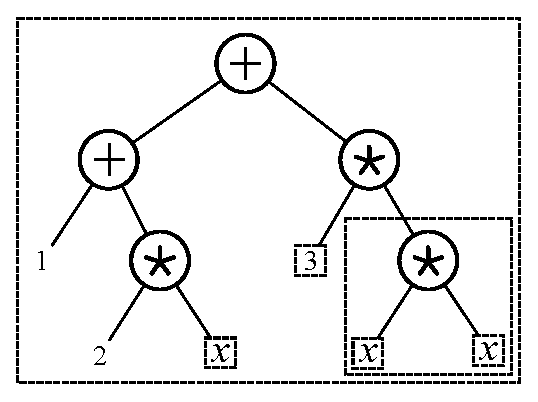
\includegraphics[width=10cm]{images/sample-polynomial.eps}
  \caption{Circuit encoding the polynomial $1 + 2x + 3x^2$ including its
    (sub--)circuits (dashed boxes)}
  \label{fig:sample-poly}
\end{figure}

The overall process is very straightforward: \JWpOne{} analyzes the polynomial
and transforms it into a circuit (the entire figure \ref{fig:sample-poly}). This
circuit is then divided to sub--circuits (every box bounded by dashes lines
except the biggest box). All the sub--circuits are then encoded in a way that
\JWpTwo{} cannot learn anything private to \JWpOne{}. To achieve that, \JWpOne{}
programs a tamper--proof hardware token with an OAFE configuration and
physically sends the token and a description of the sub--circuits to \JWpTwo{}.
After sending the circuits and the token, \JWpOne{} can shut down, it's not
needed any more.  As soon as \JWpTwo{} receives the sub--circuit description and
the token, it starts the evaluation, one sub--circuit after the other. To
discuss the evaluation the sample polynomial $1 + 2x + 3x^2$ (see figure
\ref{fig:sample-poly}) is used in the following. At this point it is
important that \JWpTwo{} does learn the degree of the polynomial $a_0 + a_1x +
a_2x^2$ but will not learn the coefficients ($a_0$, $a_1$ and $a_2$; $1$, $2$
and $3$ in the example). The first step for \JWpTwo{} is to evaluate the
sub--circuit only containing $x$. This is in fact only one sub--circuit that
appears three times in the figure. The next step would be to evaluate the
sub--circuit only encoding $3$ (remember, not learning the value $3$!), then the
sub--circuit encoding $x^2 (= x \cdot x)$ and finally the overall circuit that
encodes $1 + 2x + 3x^2$.  Usually and as in the example above, the sub--circuits
are of maximal size. A sub--circuit of maximal size is a sub--circuit into which
no additional arithmetic gates can be included. Notably, a sub--circuit can only
contain multiplications that only depend on either constants or stored
intermediate values.

To simplify the analysis of the different parts and to demonstrate the
modularity, special terms are used throughout in this thesis. A mapping from the
informal terms used above and the terms used otherwise (and defined in the
following chapters) follows:

In the informal illustration above, the encoded tuples played an important role.
They represented values and the sub--circuits evaluated to these encrypted
tuples. In fact, the sub--circuits are also twofold, they have a left and a
right side that eventually evaluate to two values: Both sides of the encrypted
tuple. For technical reasons, the two sides of the circuits and the tuples often
handled apart. They still represent the same two values encrypted with
different keys. For this reason the terms below all exist in two forms, the
\emph{Double} form (such as \emph{Double Randomized Affine Encoding}) and the
regular form (such as \emph{Randomized Affine Encoding}). At some point in the
processing, they are split syntactically, two regular entities are just the same
as one Double entity. The exact difference is not important to grasp the
procedure but it's as simple as naming tuple $\widetilde{a} = (\widetilde{a_l},
\widetilde{a_r})$ \emph{Double Value} and $\widetilde{a_l}$ and
$\widetilde{a_r}$ \emph{Value}s respectively.

\begin{itemize}

  \item The overall circuit representing exactly one function is named
    \emph{Double Affine Randomized Circuit} (DRAC) or \emph{Affine Randomized
    Circuit} (RAC)---when both sides are handled separated from each
    other---defined in chapter \ref{def:DRAC}. A DRAC is the collectivity of
    DRAEs (see next bullet point) each assigned to intermediate variables
    storing their result values.

  \item The sub--circuits are called \emph{Double Affine Randomized Encodings}
    (DRAE) and \emph{Randomized Affine Encodings} (RAE) defined in chapter
    \ref{def:DRAE}. Each (D)RAE is assigned to an intermediate variable that
    incurs in the subsequent (D)RAEs. A (D)RAE is a specification of
    calculations that have to be performed until obtaining the (D)RAEs result
    value. In terms of the (D)RAC, the result value is just an intermediate
    value that an sub--circuit evaluated to.

  \item The intermediate values that are encrypted twofoldly are named
    \emph{Double Randomized Affine Values} (DRAV), defined in chapter
    \ref{def:DRAV}.

\end{itemize}


%
% DEFINITIONS
%
\JWltwo{Definitions}
\label{sec:rae-definitions}

This chapter defines important entities that are used to define the more complex
entities in the following chapters.

% Field K
\JWlthree{Field $K$}
\label{sec:field}

\label{def:field} Throughout this thesis, $K$ represents an arbitrary large
finite field, such as $\mathbb{F}_{2^{256}}$.  When not mentioned otherwise,
this thesis assumes the field $\mathbb{F}_{2^{256}}$ specified by the
irreducible polynomial $1 + x^2 + x^5 + x^{10} + x^{256}$.


% OAFEs
\JWlthree{Oblivious Affine Function Evaluation}

The main building block of this thesis are \JWdef{Oblivious Affine Function
Evaluation}{OAFE}{s}. More precisely, \emph{Sequential one--time OAFE} as
defined by Döttling, Kraschewski and Müller--Quade \cite{davidgoliath}. The OAFE
functionality enables to sequentially evaluate $n$ affine functions specified a
priori. The OAFE functionality is implemented using the David \& Goliath
protocol and exactly one stateful tamper--proof hardware token. In other words,
one party can specify $n$ affine functions and another party will be able to
sequentially evaluate the functions exactly once respectively. The evaluating
party will only learn one evaluation of each function $f_i$ but not their
definition.

\begin{align*}
  i \in& \{1, \ldots, n\}\\
%
  f_i(x_i) = &
  a_ix_i + b_i \\
%
  = &
\begin{pmatrix}a_{i,1}\\a_{i,2}\\a_{i,3}\\\vdots\end{pmatrix}x_i +
\begin{pmatrix}b_{i,1}\\b_{i,2}\\b_{i,3}\\\vdots\end{pmatrix}
\end{align*}

\noindent{}For the sake of simplicity, the term \emph{OAFE} is used slightly
different in this thesis: The term \emph{OAFE} is used to determine a
functionality to evaluate one affine function. The plural (\emph{OAFEs}) is used
to determine a set of OAFEs that enable to evaluate a number of affine
functions. Therefore the collectivity of OAFEs as defined in this thesis can be
implemented by one \emph{Sequential one--time OAFE} functionality as defined by
Döttling, Kraschewski and Müller--Quade \cite{davidgoliath}.


%
% DUAL RANDOMIZED AFFINE VALUES
%
\JWltwo{Dual Randomized Affine Values}
\label{sec:drav}

\JWdef{Dual Randomized Affine Value}{DRAV}{s} are encrypted, signed values
representing a scalar value of the field $K$. Each DRAV is encrypted by a pair
of \emph{dual keys}. The first dual key, the \emph{static key}, remains the same
in the whole DRAC (see chapter \ref{def:DRAC}) generation procedure and is
usually denoted as $(\alpha_l, \alpha_r)$. The second dual key, the
\emph{dynamic key} is a short--lived key, usually represented as $(\beta,
\beta')$. Two DRAVs only share the same dynamic key by chance but always share
the same static key. Encoding a regular value $v \in K$ as a DRAV
$\widetilde{v}$ is straightforward: For the sake of simplicity this thesis
assumes a function $E(v)$ (also named \emph{universal encoding function}) that
is implicitly parametrized by the static dual key $(\alpha_l, \alpha_r)$ and is
able to generate a new dynamic dual key $(\beta, \beta')$ uniformly at random.
Just like $E(v)$, this thesis also assumes $D(\widetilde{v})$, named the
\emph{universal decoding function}. The universal decoding function is assumed
to be implicitly parametrized by the encryption keys from the context it is
used. Both functions are defined below.  The universal encoding and decoding
functions only serve the purpose of describing the methodology. In the reality
especially the function $D$ is never called by anyone. That would not even be
possible since only the party in possession of the keys (\JWpOne{}) has the
information to do so but because of the non--interactivity of the protocol,
\JWpOne{} is not active anymore when the second party (not in possession of the
keys, usually named \JWpTwo{}) starts the evaluation. The real protocol encodes
the encryption and decryption into the OAFEs in a way that as soon as \JWpTwo{}
tries to cheat everything eventually becomes uniform randomness. This is done
using carefully chosen linear functions realized as OAFEs. The setup of these
linear functions assures the addition of uncorrelated uniform randomness as soon
as \JWpTwo{} tries to cheat. One can envision the process as applying a
one--time pad encryption that is only correctly removed if the other party did
not try to cheat. As soon as the second party tries to cheat this resembles the
attempt to undo a one--time pad encryption using another one--time pad. This
clearly leads to a one--time pad encryption which can only be undone using an
unknown one--time pad. The unknown one--time pad is a composition of the
encrypting one--time pad and the one--time pad using which the decryption was
attempted.

\begin{align}
  \label{eqn:one-time-pad}
  \hat{E}(v; \alpha_l, \alpha_r, \beta, \beta') &=
  (\alpha_l \cdot v + \beta, \alpha_r \cdot v + \beta')\\
  %
  E(v) &= \hat{E}(v; \alpha_l, \alpha_r, \beta, \beta') \qquad
  \text{(implicitly knowing the keys)}\nonumber
  %
\end{align}

\noindent{}The values $\beta$ and $\beta'$ are as mentioned above fresh values
uniformly at random. In finite fields $\beta$ and $\beta'$ therefore one--time
encrypt both tuple components. As such a DRAV is one--time pad encrypted.
$\alpha_l$ and $\alpha_r$ are also values uniformly at random but are in
contrast to $\beta$ and $\beta'$ used in for DRAVs throughout the whole
process. The purpose they serve will be discussed in the following chapters.

Notationally, the DRAV encoding a scalar value $v$ is usually denoted as
$\widetilde{v}$. $\widetilde{v}$'s tuple components are usually referred to as
$\widetilde{v_l}$ and $\widetilde{v_r}$: $(\widetilde{v_l}, \widetilde{v_r}) =
\widetilde{v} = E(v)$. Where appropriate, DRAVs are also denoted in a vector
notation $\begin{pmatrix}\widetilde{v_l}\\\widetilde{v_r}\end{pmatrix} \hat{=}
(\widetilde{v_l}, \widetilde{v_r}) = E(v)$. The universal decoding function
$D(\widetilde{v})$ is defined as:

\begin{align}
  %
  \hat{D}(\widetilde{v}; \alpha_l, \alpha_r, \beta, \beta') &=
  \begin{pmatrix}
    \frac{\widetilde{v_l} - \beta}{\alpha_l}\\
    \frac{\widetilde{v_r} - \beta'}{\alpha_r}
  \end{pmatrix} \nonumber\\
  %
  \label{eqn:keys-assumed}
\begin{pmatrix}D_l(\widetilde{v})\\D_r(\widetilde{v})\end{pmatrix} &=
  \hat{D}(\widetilde{v}; \alpha_l, \alpha_r, \beta, \beta') \qquad
  \text{(implicitly knowing the keys)}\\
  %
  D(\widetilde{v}) &=
  \left\{
    \begin{array}{l l}
      D_l(\widetilde{v}) & \quad
      \text{if}~D_l(\widetilde{v}) = D_r(\widetilde{v})\\
      \bot & \quad \text{otherwise ($\widetilde{v}$ is non--well--formed)}\\
    \end{array}\right.\nonumber
    %
\end{align}

\noindent{}In equation \ref{eqn:keys-assumed} one can see that the universal
decoding function $D$ assumes context--specific  dual keys $(\alpha_l,
\alpha_r)$ and $(\beta, \beta')$. If an attacker at some point passes a DRAV
that is not expected to be decoded at this point, the decoding will fail and
evaluate to $\bot$. This is evident because $D$ will decode using the dual keys
of the DRAV that was expected to be decoded (see also Lemma
\ref{lem:well-formed-fun-of-dec-fun}).

\begin{lem}
  \label{lem:DRAV-random}

  A party that is not in possession of the encryption (dual) keys will not learn
  anything from a DRAV. A DRAV is a tuple consisting of two values uniformly at
  random that is uncorrelated to any other DRAV.

\end{lem}
\begin{proof}

  In a finite field, the addition of some value $r$ uniformly at random to
  another value $x \in K$ is uniformly at random. Therefore $\alpha_l \cdot v +
  \beta$ and $\alpha_r \cdot v + \beta'$ are two values uniformly at random if
  and only if $\beta$ and $\beta'$ are uniformly at random. Per definition,
  every time a DRAV gets encoded, $\beta$ and $\beta'$ are fresh uniformly
  distributed random values. Trivially, a DRAV is therefore uncorrelated to any
  other DRAV.

\end{proof}


% WELL-FORMED DRAVs
\JWlthree{Well--Formed DRAVs}

A DRAV $\widetilde{v}$ is well--formed iff $D(\widetilde{v}) \neq \bot$.
Therefore, if $D(\widetilde{\chi}) = \bot$, $\chi$ is non--well-formed.
Obviously the well--formedness of a DRAV depends on the encryption keys used to
decrypt. Decoding well--formed DRAVs using any other decoding function will
lead to $\bot$ because the well--formed DRAV looks non--well--formed to the
other decoding function.

\begin{lem}
  \label{lem:well-formed-fun-of-dec-fun}

  DRAV well--formedness is a function of the keys used to decrypt it.

\end{lem}
\begin{proof}

  Assuming two well--formed DRAVs $\widetilde{a}$ and $\widetilde{b}$. Both
  DRAVs have their respective decoding function $D^a$ and $D^b$ and their
  dynamic dual key (say $(\beta_1, \beta_2)$ for $\widetilde{a}$ and
  $(\beta_3, \beta_4)$ for $\widetilde{b}$). The following equations demonstrate
  the decoding of the DRAVs $\widetilde{a}$ and $\widetilde{b}$ with the correct
  keys and the wrong keys respectively.

  \begin{align*}
    %
    D^a(\widetilde{a}) &= D(\widetilde{a}) \qquad\text{(using $\widetilde{a}$'s
    keys)}\\
    %
    D^b(\widetilde{b}) &= D(\widetilde{b}) \qquad\text{(using $\widetilde{b}$'s
    keys)}\\
    %
    a &= D^a(\widetilde{a}) \hat{=}
    \begin{pmatrix}
      \frac{(\alpha_l \cdot a + \beta_1) - \beta_1}{\alpha_l}\\
      \frac{(\alpha_r \cdot a + \beta_2) - \beta_2}{\alpha_r}\\
    \end{pmatrix}
    = a\\
    %
    a' &= D^a(\widetilde{b}')
    \hat{=}
    \begin{pmatrix}
      \frac{(\alpha_l \cdot b + \beta_3) - \beta_1}{\alpha_l}\\
      \frac{(\alpha_r \cdot b + \beta_4) - \beta_2}{\alpha_r}\\
    \end{pmatrix}
    \hat{=}
    \begin{pmatrix}
      b +
      \frac{\beta_3 - \beta_1}{\alpha_l}\\
      b +
      \frac{\beta_4 - \beta_2}{\alpha_r}\\
    \end{pmatrix}
    \stackrel{*}{=} \bot\\
    %
    b &= D^b(\widetilde{b}) \hat{=}
    \begin{pmatrix}
      \frac{(\alpha_l \cdot b + \beta_3) - \beta_3}{\alpha_l}\\
      \frac{(\alpha_r \cdot b + \beta_4) - \beta_4}{\alpha_r}\\
    \end{pmatrix}
    = b\\
    %
    b' &= D^b(\widetilde{a}')
    \hat{=}
    \begin{pmatrix}
      \frac{(\alpha_l \cdot a + \beta_1) - \beta_3}{\alpha_l}\\
      \frac{(\alpha_r \cdot a + \beta_2) - \beta_4}{\alpha_r}\\
    \end{pmatrix}
    \hat{=}
    \begin{pmatrix}
      a +
      \frac{\beta_1 - \beta_3}{\alpha_l}\\
      a +
      \frac{\beta_2 - \beta_4}{\alpha_r}\\
    \end{pmatrix}
    \stackrel{*}{=} \bot\\
    %
    &\JWnegl{}
  \end{align*}

  \noindent{}As one can see decoding a well--formed DRAV using the wrong
  decoding function leads to $\bot$.

\end{proof}


\begin{lem}
  \label{lem:DRAV-indistinguishable}

  Without knowing the encryption keys, a non--well--formed DRAV is
  indistinguishable from a well--formed DRAV.

\end{lem}
\begin{proof}

  From Lemma \ref{lem:DRAV-random} we learn, that a well--formed DRAV only
  consists of two values uniformly at random. From Lemma
  \ref{lem:well-formed-fun-of-dec-fun} we learn, that well--formedness is a
  function of the encryption keys used to eventually decrypt the DRAV. Since a
  party that is not in possession of the encryption keys cannot know the
  decryption function, well--formed and non--well--formed DRAVs are
  indistinguishable for a party not in possession of the keys.
\end{proof}


% DIRECT DRAV ARITHMETIC
\JWlthree{Direct DRAV Addition}
\label{sec:DRAV-addition}

This thesis referres to DRAV addition as \emph{direct DRAV addition} because is
has the property that it can be performed without knowledge of a DRAV's
encryption keys. But (see Lemma \ref{lem:wrong-add}) the addition of DRAVs does
not lead to additional information. Although direct DRAV addition can be
performed without the knowledge of a party in possession of the keys, this will
not reveal additional information or cheating options. Since direct DRAV
additions do automatically generate new encryption keys, the result will only be
well--formed iff the addition was intended by the party in possession of the
keys (see Lemma \ref{lem:well-formed-fun-of-dec-fun}).

\begin{lem}
  \label{lem:DRAV-add}

Additions commissioned by a party in possession of the encryption keys of
well--formed DRAVs lead to well--formed DRAV: $\widetilde{x} =
(\widetilde{x_l}, \widetilde{x_r})$ and $\widetilde{y} = (\widetilde{y_l},
\widetilde{y_r})$ can be added component--wise to $\widetilde{z} =
\left(\widetilde{x_1} + \widetilde{y_1}, \widetilde{x_2} +
\widetilde{y_2}\right)$. The encryption keys for $\widetilde{z}$ will be
$(\alpha_l, \alpha_r)$ and $(\beta_1 + \beta_3, \beta_2 + \beta_4)$ assuming
$\widetilde{x}$ was encrypted with $(\alpha_l, \alpha_r)$ and $(\beta_1,
\beta_2)$ and $y$ was encrypted with $(\alpha_l, \alpha_r)$ and $(\beta_3,
\beta_4)$.

\end{lem}
\begin{proof}

From ($\widetilde{x} = \left(\alpha_l \cdot x + \beta_1,
\alpha_r \cdot x + \beta_2\right)$, $\widetilde{y} = \left(\alpha_l \cdot x +
\beta_3, \alpha_r \cdot x + \beta_4\right)$) it's obvious that: $\widetilde{z} =
\left(\alpha_l \cdot (x+y) + (\beta_1 + \beta_3), \alpha_r \cdot (x+y) +
(\beta_2 + \beta_4)\right)$ and $\widetilde{z}$ is well--formed.

\end{proof}

\begin{lem}
  \label{lem:DRAV-add-bad}

The addition to a non--well--formed DRAV leads to a non--well--formed DRAV. It's
of particular interest the following property holds: $\forall \widetilde{x}:
\widetilde{x} + \bot = \bot + \widetilde{x} = \bot$.

\end{lem}
\begin{proof}

Let $\widetilde{\chi}$ be a non--well--formed DRAV, so: $\widetilde{\chi} =
(\alpha_l \cdot \chi + \beta_3 + \Delta_l, \alpha_r \cdot \chi + \beta_4 +
\Delta_r)$. The component--wise addition $\widetilde{\nu}$ of $\widetilde{\chi}$
to any well--formed $\widetilde{x} = (\alpha_l \cdot x + \beta_1, \alpha_r \cdot
x + \beta_2)$ is $\widetilde{\nu} = (\alpha_l \cdot (x+\chi) + (\beta_1+\beta_3)
+ \Delta_l, \alpha_r \cdot (x+\chi) + (\beta_2+\beta_4) + \Delta_r)$.  Using the
component--wise universal decoding functions $D_l(\widetilde{v})$ and
$D_r(\widetilde{v})$ (see chapter \ref{def:DRAV}), the value of $\chi$ is $\chi
= (D_l(\widetilde{\chi_l}), D_r(\widetilde{\chi_r})) = (x + \chi +
\frac{\Delta_l}{\alpha_l}, x + \chi + \frac{\Delta_r}{\alpha_r})$. So: $\forall
(\Delta_r, \Delta_l) \in K \setminus \{(0, 0)\} \wedge \frac{\Delta_l}{\alpha_l}
\neq \frac{\Delta_r}{\alpha_r}: D(\widetilde{\chi}) = \bot$. Since the
encryption keys are not known to an attacker, $\frac{\Delta_l}{\alpha_l} \neq
\frac{\Delta_r}{\alpha_r}$ holds except for a negligible probability if
$\Delta_r \neq 0 \vee \Delta_r \neq 0$ and that's the property for being forged
(non--well--formed) which was the assumption. Trivially $\bot + \bot = \bot$ by
a similar argument.

\end{proof}


\begin{lem}
  \label{lem:wrong-add}

  An addition that was unintended by a party in possession of the encryption
  keys will not reveal additional information. A party that is not in possession
  of the keys but that knows three well--formed DRAVs $\widetilde{a}$,
  $\widetilde{b}$ and $\widetilde{c}$ that is commissioned to execute the
  addition $\widetilde{y} = \widetilde{a} + \widetilde{b}$ cannot generate a
  well--formed DRAV $\widetilde{y}' = \widetilde{a} + \widetilde{c}$.

\end{lem}

\begin{proof}

  Since every DRAV has per definition different dynamic keys the
  component--wise addition of two DRAVs leads to a new dynamic key that is
  characteristic for the addition intended by a party in possession of the
  encryption keys.

  Assuming there are three well--formed DRAVs $\widetilde{a}$, $\widetilde{b}$
  and $\widetilde{c}$ and the party in possession of the keys commissions any
  other party to execute $\widetilde{y} = \widetilde{a} + \widetilde{b}$ but the
  other party tries to illicitly execute $\widetilde{y}' = \widetilde{a} +
  \widetilde{c}$:

  \begin{align*}
    %
    \widetilde{a} &=
    \begin{pmatrix}
      \alpha_l \cdot a + \beta_1\\
      \alpha_r \cdot a + \beta_2
    \end{pmatrix}\\
    %
    \widetilde{b} &=
    \begin{pmatrix}
      \alpha_l \cdot b + \beta_3\\
      \alpha_r \cdot b + \beta_4
    \end{pmatrix}\\
    %
    \widetilde{c} &=
    \begin{pmatrix}
      \alpha_l \cdot c + \beta_5\\
      \alpha_r \cdot c + \beta_6
    \end{pmatrix}\\
    %
    \widetilde{y} &=
    \begin{pmatrix}
      \alpha_l \cdot a + \beta_1 + \alpha_l \cdot b + \beta_3\\
      \alpha_r \cdot a + \beta_2 + \alpha_r \cdot b + \beta_4\\
    \end{pmatrix} =
    \begin{pmatrix}
      \alpha_l \cdot (a+b) + (\beta_1 + \beta_3)\\
      \alpha_r \cdot (a+b) + (\beta_2 + \beta_4)\\
    \end{pmatrix}\\
    %
    \widetilde{y}' &=
    \begin{pmatrix}
      \alpha_l \cdot a + \beta_1 + \alpha_l \cdot c + \beta_5\\
      \alpha_r \cdot a + \beta_2 + \alpha_r \cdot c + \beta_6\\
    \end{pmatrix} =
    \begin{pmatrix}
      \alpha_l \cdot (a+c) + (\beta_1 + \beta_5)\\
      \alpha_r \cdot (a+c) + (\beta_2 + \beta_6)\\
    \end{pmatrix}\\
    %
  \end{align*}

  As soon as the party in possession of the keys tries to decode using the
  encryption keys for $\widetilde{y}$ the result (either $\widetilde{y}$ or
  $\widetilde{y}'$) the other party will get caught if it tried to cheat:

  \begin{align*}
    %
    D^y(\widetilde{y}) &= D(y) \qquad\text{(using $y$'s encryption keys)}\\
    %
    y &= D^y(\widetilde{y}) \hat{=}
    \begin{pmatrix}
      \frac{(\alpha_l \cdot (a+b) + (\beta_1 + \beta_3)) - (\beta_1+\beta_3)}
           {\alpha_l}\\
      \frac{(\alpha_r \cdot (a+b) + (\beta_2 + \beta_4)) - (\beta_2+\beta_4)}
           {\alpha_r}\\
    \end{pmatrix}
    = a+b\\
    %
    y' &= D^y(\widetilde{y}')
    \hat{=}
    \begin{pmatrix}
      \frac{(\alpha_l \cdot (a+b) + (\beta_1 + \beta_5)) - (\beta_1+\beta_3)}
           {\alpha_l}\\
      \frac{(\alpha_r \cdot (a+b) + (\beta_2 + \beta_6)) - (\beta_2+\beta_4)}
           {\alpha_r}\\
    \end{pmatrix}
    \hat{=}
    \begin{pmatrix}
      (a+b) +
      \frac{\beta_5 - \beta_3}{\alpha_l}\\
      (a+b) +
      \frac{\beta_6 - \beta_4}{\alpha_r}\\
    \end{pmatrix}
    \stackrel{*}{=} \bot\\
    %
    &\JWnegl{}
  \end{align*}
\end{proof}


% FINAL DRAV DECODING
\JWlthree{Final DRAV Decoding}
\label{sec:drav-final-decoding}

Finally decoding a DRAV means to extract the hidden value which is crucial
because otherwise everything else would be useless. It can be trivially done
using the universal decoding function $D(\widetilde{v})$. But as the encryption
keys, $D$ is not available to ordinary parties. This chapter describes a system
that enables the party in possession of the keys to allow other parties to
decode a specific DRAV. Usually it only allows the final DRAV to be decoded,
otherwise intermediate information would leak.

The overall costs thereof are only one addition and an OAFE call for the
ordinary party. Of course, the OAFE has to be set up by the party that knows the
encryption keys. The setup of this OAFE can be seen as the authorization to
decode exactly one specific DRAV. The procedure will decode a DRAV to a final
scalar value although $D$ is a partial function. The special value $\bot$ that
$D$ evaluates to if the DRAV is non--well--formed is simply mapped to uniform
randomness. As a result of Lemma \ref{lem:well-formed-fun-of-dec-fun}, a DRAV is
also non--well--formed if the encryption keys differ from the keys of the DRAV
whose decoding was intended. Therefore, no other DRAVs can be decoded
illegitimately. In the following, the DRAV to be decoded is named $\widetilde{v}
= (\widetilde{v_1}, \widetilde{v_2})$ and the OAFE permitting the decoding is
called the \emph{final OAFE}.

The second party's input to the final OAFE is $\widehat{v} = \widetilde{v_1} +
\widetilde{v_2}$, the addition of both components of the DRAV to decode.  The
final OAFE was set up by the first party as follows: Assuming $\widetilde{v}$ is
encrypted by $(\alpha_l, \alpha_r)$ and $(\beta_1, \beta_2)$ the first party
knows $\widehat{v}$ has to be encrypted using $(\alpha_l + \alpha_r)$ and
$(\beta_1 + \beta_2)$.  Given this knowledge the final OAFE setup is
$\frac{1}{\alpha_l + \alpha_r} \cdot \widehat{v} - \frac{\beta_1 +
\beta_2}{\alpha_l + \alpha_r}$.

Again, it's important that an attacker is getting caught when trying to forge a
DRAV ($D(\widetilde{v}) = \bot$ if $\widetilde{v}$ has been forged, $\bot$ is
mapped to uniform randomness in this process since an OAFE has no
$\bot$--value). If the attacker cheated somewhere in the process and forged one
of the DRAV tuples $\widetilde{x} = (\widetilde{x_1}, \widetilde{x_2})$ to
$\widetilde{x'} = (\widetilde{x_1} + \Delta_1, \widetilde{x_2} + \Delta_2)$, the
DRAV $\widetilde{x'}$ becomes---except for a negligible
probability---non--well--formed (see section \ref{sec:drav}). The result is that
the decoded result will become uniform randomness (assuming $\widetilde{x}$ is
forged to $\widetilde{x'_1} = \widetilde{x_1} + \Delta_1$ and $\widetilde{x'_2}
= \widetilde{x_2} + \Delta_2$):

\begin{align*}
  \widehat{x'} = & \widetilde{x'_1} + \widetilde{x'_2} = \widetilde{x_1} +
  \Delta_1 + \widetilde{x_2} + \Delta_2 \\
  %
  \Rightarrow x' = & \frac{1}{\alpha_l + \alpha_v} \cdot \widehat{x'} -
  \frac{\beta_{x_1} +
  \beta_{x_2}}{\alpha_l + \alpha_v} \\
  %
  \Leftrightarrow x' = & \frac{\widetilde{x_1} + \Delta_1 +
  \widetilde{x_2} + \Delta_2}{\alpha_l + \alpha_v} -
  \frac{\beta_{x_1} +\beta_{x_2}}{\alpha_l + \alpha_v}\\
  %
  \Leftrightarrow x' = & \frac{(\alpha_l x + \beta_{x_1}) + \Delta_1 +
  (\alpha_v x + \beta_{x_2}) + \Delta_2}{\alpha_v + \alpha_l} -
  \frac{\beta_{x_1} +\beta_{x_2}}{\alpha_l + \alpha_v} \\
  %
  \Leftrightarrow x' = & \frac{(\alpha_l+\alpha_v)x + (\beta_{x_1}+\beta_{x_2} +
  \Delta_1+\Delta_2)}{\alpha_l+\alpha_v} -
  \frac{\beta_{x_1} +\beta_{x_2}}{\alpha_l + \alpha_v} \\
  %
  \Leftrightarrow x' = & x + \frac{\beta_{x_1}+\beta_{x_2}}{\alpha_l+\alpha_v}
  + \frac{\Delta_1 + \Delta_2}{\alpha_l + \alpha_v} -
  \frac{\beta_{x_1}+\beta_{x_2}}{\alpha_l + \alpha_v} \\
  %
  \Leftrightarrow x' = & x + \frac{\Delta_1 + \Delta_2}{\alpha_l + \alpha_v}\\
\end{align*}

Because an attacker is not in possession of the static encryption keys
$\alpha_l$ and $\alpha_r$, it cannot control the value of $\frac{\Delta_1 +
\Delta_2}{\alpha_l + \alpha_r}$. Since $\alpha_l$ and $\alpha_r$ are chosen
uniformly at random, the result $x'$ becomes uniformly at random, too. An
attacker could choose $\Delta_l + \Delta_r = 0$ but that would not change the
result at all because it added both components before using the final OAFE.


%
% DUAL RANDOMIZED AFFINE ENCODING
%
\JWltwo{Dual Randomized Affine Encoding}
\label{sec:drae}

\JWdef{Dual Randomized Affine Encoding}{DRAE}{s} are affine representations of
parts of arithmetic circuits. A DRAE describes arithmetic expressions in terms
of affine functions without revealing the original expression. A single DRAE
alone is not powerful enough to describe arbitrary complex arithmetic
expressions, therefore chapter \ref{def:DRAC} proposes a procedure to evaluate
arbitrary expression using multiple DRAEs. Technically, a DRAE is a
specification of calculations that need to be performed to eventually obtain the
evaluated value of the arithmetic expression. The reason for using DRAEs instead
of evaluating the arithmetic expressions as usual is that a DRAE operates on
encrypted values. Both, the input values and the output value of a DRAE are
DRAVs (see chapter \ref{def:DRAV}). Additionally, the arithmetic expression
performed is hidden from every party that is not in possession of the encryption
keys.  The reason why DRAEs specify the calculations using affine functions is
that OAFEs provide a secure way to obliviously evaluate affine functions. The
procedure of evaluating arithmetic expression using DRAEs works as follows: The
first party that is in possession of the encryption keys chooses the expression
to evaluate.  Next, it sets up the DRAE but hides the affine calculations inside
OAFEs. In fact, instead of the affine calculations themselves, the DRAEs
specifies references to the OAFEs that were configured to evaluate these
functions obliviously. The evaluating party finally evaluates the DRAEs with the
help of the OAFEs provided by the first party.

To easily envision the role of DRAEs and DRAVs, given a number of DRAVs, a DRAE
performs some arithmetic operations on them and evaluates to a DRAV. Just the
same way given a number of values, an arithmetic expression evaluates to a value
(e.g. given $x=17$ and $y=23$, the arithmetic expression $x*y + 3$ evaluates to
$394$).

Summing up, DRAE evaluation is partitioning calculations between the two
parties: The first that builds the DRAE and sets up the OAFEs and the second
that provides the input and does the evaluation. In fact, the first party isn't
directly involved in the evaluation process, it provided its calculations a
priori hidden inside OAFEs. But as stated above, one DRAE cannot realize
arbitrary complex arithmetic expressions, as a rule of thumb: As soon as a
(non--trivial) multiplication is part of the original arithmetic, one DRAE is
not enough to evaluate it.


% FORMAL DESCRIPTION
\JWlthree{Formal Description}

Because DRAEs are tightly related to DRAVs, they fulfill similar properties:

\begin{enumerate}

  \item \label{prop:drae-encrypted} DRAEs are encrypted: Without the encryption
    keys, they don't reveal any information.

  \item \label{prop:drae-signed} DRAEs are signed: If someone tries to forge a
    DRAE, it will become non--well--formed and operations with that DRAE result
    in non--well--formed DRAEs.

  \item DRAEs are not exchangeable with other DRAEs. If an attacker tries to
    provide a DRAE that was not intended by the party in possession of the keys,
    all following DRAEs will evaluate to uniform randomness.

  \item \label{prop:drae-oafe} DRAEs can be securely evaluated using OAFEs.

  \item \label{prop:drae-not-enough} DRAEs can not express arbitrary arithmetic
    circuits alone.

\end{enumerate}

\noindent{}Informally, a DRAE is composed of two finite multi--sets and a
constant DRAV. The first multi--set, called the \emph{multiplicative terms}
contains tuples of computations. The second multi--set, called the
\emph{additive terms} contains computations that can be evaluated to DRAVs. The
constant DRAV represents the constant terms in the arithmetic expression. The
component--wise multiplication of each of the computation tuples (from the
multiplicative terms) yields DRAVs, too. The sum of the constant DRAV, the DRAVs
obtained from the additive terms and the DRAVs obtained from the multiplicative
terms is the evaluated value of this DRAE. Again the evaluated value is a valid
DRAV.

More formally, a DRAE can be described as follows where
$\mathcal{E}_\mathcal{C}$ represents the DRAEs, $\mathcal{C}$ the affine
computations, $\mathcal{V}$ the set of all DRAVs and $\mathcal{V}_\mathcal{C}$
the computations that lead to DRAVs.

\begin{align}
%
  &\text{The static keys } \alpha_l, \alpha_r \in K \setminus \{0\} \nonumber\\
%
  &\text{The dynamic keys } \beta, \beta' \in K \nonumber\\
%
  &s, x, x', i \in K \nonumber\\
%
  \mathcal{C} = & \{ c(x) = s \cdot x + i \} \nonumber\\
%
  \mathcal{V}_\mathcal{C} = & \{ (\alpha_l \cdot f(x) + \beta,
                      \alpha_r \cdot f'(x') + \beta' )
                    \mid f, f' \in \mathcal{C} \} \nonumber\\
%
  \label{rel:DRAE}
  \mathcal{E}_\mathcal{C} = & \{ (M, A, k) \mid
      M \subseteq \mathcal{V}_\mathcal{C} \times
      \mathcal{V}_\mathcal{C}; A \subseteq \mathcal{V}_\mathcal{C};
      k \in \mathcal{V};
      A, M~\text{finite multi--sets} \}
%
\end{align}

As stated in the introduction to this chapter, the calculations are hidden
inside OAFEs. When the party that built the DRAE transmits it to the evaluating
party, it obviously replaces the concrete affine computations by references to
the OAFEs that calculate them obliviously.  Because of the definition of OAFEs
(see chapter \ref{def:OAFE}) the evaluating party will only learn exactly one
evaluation $c(x)$ for each variable $x$. A \emph{pre--evaluated DRAE} is defined
as the entity that the evaluating party obtains after successfully having
evaluated all the computations (using the OAFEs). The pre--evaluated DRAEs
($\mathcal{E}$) are defined as follows:

\begin{align}
  \mathcal{V} = & \{ (v_l, v_r) \mid v_l, v_r \in K \}
  &\text{, the DRAVs (chapter \ref{def:DRAV})} \nonumber\\
%
  \label{rel:pre-eval-DRAE}
  \mathcal{E} = & \{ (M, A, k) \mid
      M \subseteq \mathcal{V} \times \mathcal{V};
      A \subseteq \mathcal{V};
      k \in \mathcal{V} \}
      &\text{, the pre--evaluated DRAEs}
\end{align}


% DECODING DRAEs
\JWlthree{Decoding DRAEs}
\label{sec:DRAE-decoding}

Entirely evaluating a pre--evaluated DRAE to obtain the DRAV is straightforward:
A pre--evaluated DRAE $e \in \mathcal{E} = (M,A, k)$ can be evaluated to its
single resulting DRAV $r \in \mathcal{V}$ as follows (all additions performed
component--wise):

\begin{align*}
M' &= \Bigg\{ m_1 \cdot m_2\ \Bigg|\ \begin{pmatrix}m_1\\m_2\end{pmatrix}
\in M \Bigg\} \\
r & = \sum_{a \in A}a + \sum_{m \in M'}m + k
\end{align*}


% DRAE ARITHMETIC
\JWlthree{DRAE Arithmetic}

The purpose of DRAEs is to specify arithmetic operations. This chapter describes
how arithmetic operations can be safely encoded using DRAEs. Since DRAEs
evaluate to DRAVs and DRAVs can be easily added (see chapter
\ref{sec:DRAV-addition}), DRAE addition is easy, too: A DRAE that encodes the
addition of two DRAEs can be built practically costless. But DRAE multiplication
is slightly more complex: To multiply two arbitrary DRAEs, both DRAEs have to be
evaluated separately, their results have have to be assigned to intermediate
variables and a third DRAE has to be built that solely multiplies the
intermediate variables. In contrast to general DRAE multiplication, a DRAE can
encode the multiplication of two DRAVs and assigning intermediate values to
variables is just giving intermediate DRAVs a temporary name.


%Direct Addition
\JWlfour{Addition}
\label{sec:DRAE-addition}

Since two DRAVs can directly be added as explained in chapter
\ref{sec:DRAV-addition}, two DRAEs can be added by concatenating the
multiplicative ($M$ in relations \ref{rel:DRAE} and \ref{rel:pre-eval-DRAE}) and
additive ($A$) terms. Notably, although the encryption keys change, this
operation can be performed by any party, in possession of the encryption keys or
not. Similarly to DRAVs, unintended operations ruin the information because the
encryption keys change when performing operations. Operations unintended by the
party in possession of the keys lead to non--well--formed DRAVs because wrong
encryption keys will be used to decode them.


%Multiplication
\JWlfour{Multiplication}
\label{sec:DRAE-multiplication}

Since neither a DRAV (chapter \ref{def:DRAV}) nor a DRAE (see above) can be
multiplied directly, most multiplications have to be performed using a
construction involving additional DRAEs and intermediate variables holding
DRAVs. Chapter \ref{def:DRAC} describes the transformation of arbitrary
arithmetic expression. This chapter describes multiplications that can directly
be expressed as a DRAE: A single multiplication of two DRAVs $\widetilde{x}$ and
$\widetilde{y}$ (each assigned to a variable) to a DRAE $E \in \mathcal{E}$.

\JWtodo{Warum müssen sie gemixt werden: Das Argument mit gegen
Null prüfen}

\JWtodo{Das Mixen genauer erklären}


\begin{align*}
  E & \in \mathcal{E}; \widetilde{x}, \widetilde{y} \in \mathcal{V};
  r_1, r_2, r_3, r_4, r_5, r_6, r_7, r_8 \in K;
  \alpha_l, \alpha_r \in K \setminus \{0\} \\
  %
  E & = \widetilde{x} \otimes \widetilde{y} \\
  %
  E & = \Bigg(\left\{\left(
            \begin{pmatrix}
              \alpha_l \cdot D_l(\widetilde{x}) - r_1 \\
              \alpha_r \cdot D_r(\widetilde{x}) - r_5
            \end{pmatrix},
            \begin{pmatrix}
              1        \cdot D_l(\widetilde{y}) - r_2 \\
              1        \cdot D_r(\widetilde{y}) - r_6
            \end{pmatrix}
        \right)\right\}, \\
    &   \qquad\bigg\{
        \begin{pmatrix}
            \alpha_lr_2 \cdot D_r(\widetilde{x}) + r_3 \\
            \alpha_rr_6 \cdot D_l(\widetilde{x}) + r_7
          \end{pmatrix} \\
    &  \qquad,
        \ \begin{pmatrix}
            r_1        \cdot D_r(\widetilde{y}) + r_4 \\
            r_5        \cdot D_l(\widetilde{y}) + r_8
          \end{pmatrix}
        \bigg\} \\
    &  \qquad, 0
        \Bigg) \\
\end{align*}

In the relation above, the first curly bracket contains the multiplicative
terms, the second contains the additive terms and the constant is set to $0$
since no constant addition is performed.

The following equations demonstrate that the multiplication of two well--formed
DRAVs will evaluate to the desired result. Additionally is shows that a
non--well--formed DRAV operands will turn the result to a non--well--formed DRAV
as well. In the following the decoding of a DRAE will be analyzed and it will
become apparent that every DRAV modification propagates through a
multiplication. The DRAE $E$ gets decoded (as defined in chapter
\ref{sec:DRAE-decoding}) to a DRAV $\widetilde{e}$.

\begin{align*}
  \widetilde{e} & =
  \begin{pmatrix}
    (\alpha_l D_l(\widetilde{x})-r_1)
    (         D_l(\widetilde{y})-r_2) \\
    (\alpha_r D_r(\widetilde{x})-r_5)
    (         D_r(\widetilde{y})-r_6)
  \end{pmatrix}
  +
  \begin{pmatrix}
    \alpha_lr_2 D_r(\widetilde{x}) + r_3 +
    r_1         D_r(\widetilde{y}) + r_4 \\
    \alpha_rr_6 D_l(\widetilde{x}) + r_7 +
    r_5         D_l(\widetilde{y}) + r_8
  \end{pmatrix} \\
%
  & =
  \begin{pmatrix}
    \alpha_l     D_l(\widetilde{x}) D_l(\widetilde{y})
    -\alpha_lr_2 D_l(\widetilde{x})
    -r_1         D_l(\widetilde{y})
    +r_1r_2 \\
    \alpha_r     D_r(\widetilde{x}) D_r(\widetilde{y})
    -\alpha_rr_6 D_r(\widetilde{x})
    -r_5         D_r(\widetilde{y})
    +r_5r_6
  \end{pmatrix} \\
  &\ \ \ +
  \begin{pmatrix}
    \alpha_lr_2 D_r(\widetilde{x}) + r_3 +
    r_1         D_r(\widetilde{y}) + r_4 \\
    \alpha_rr_6 D_l(\widetilde{x}) + r_7 +
    r_5         D_l(\widetilde{y}) + r_8
  \end{pmatrix} \\
%
  & =
  \begin{pmatrix}
    \alpha_l     \left(x + \frac{\Delta_1}{\alpha_l}\right)
                 \left(y + \frac{\Delta_3}{\alpha_l}\right)
    -\alpha_lr_2 \left(x + \frac{\Delta_1}{\alpha_l}\right)
    -r_1         \left(y + \frac{\Delta_3}{\alpha_l}\right)
    +r_1r_2 \\
    \alpha_r     \left(x + \frac{\Delta_2}{\alpha_r}\right)
                 \left(y + \frac{\Delta_4}{\alpha_r}\right)
    -\alpha_rr_6 \left(x + \frac{\Delta_2}{\alpha_r}\right)
    -r_5         \left(y + \frac{\Delta_4}{\alpha_r}\right)
    + r_5r_6
  \end{pmatrix} \\
  &\ \ \ +
  \begin{pmatrix}
    \alpha_lr_2  \left(x + \frac{\Delta_2}{\alpha_r}\right) + r_3 +
    r_1          \left(y + \frac{\Delta_4}{\alpha_r}\right) + r_4 \\
    \alpha_rr_6  \left(x + \frac{\Delta_1}{\alpha_l}\right) + r_7 +
    r_5          \left(y + \frac{\Delta_3}{\alpha_l}\right) + r_8
  \end{pmatrix} \\
%
  & =
  \begin{pmatrix}
    \alpha_l(xy) + (r_1r_2 + r_3 + r_4)
    + \Delta_3x + \Delta_1y
    + \frac{\Delta_1\Delta_3}{\alpha_l}
    - \Delta_1r_2
    + \frac{\Delta_2\alpha_lr_2}{\alpha_r}
    - \frac{\Delta_3r_1}{\alpha_l}
    + \frac{\Delta_4r_1}{\alpha_r}
    \\
    \alpha_r(xy) + (r_5r_6 + r_7 + r_8)
    + \Delta_4x + \Delta_2y
    + \frac{\Delta_2\Delta_4}{\alpha_r}
    + \frac{\Delta_1\alpha_lr_6}{\alpha_l}
    - \Delta_2r_6
    + \frac{\Delta_3r_5}{\alpha_l}
    - \frac{\Delta_4r_5}{\alpha_r}
  \end{pmatrix} \\
%
\end{align*}

\noindent{}That leads to two possibilities: Either $E$ is well--formed or not.
Although the DRAVs $\widetilde{x}$ and $\widetilde{y}$ are both used in multiple
affine expression, it is safe to assume they have the same value. At the first
glance, one could think a malicious adversary could use different values for the
same variable. But since all expressions depending on the same variable are
evaluated using one and the same OAFE, the attacker has to commit itself to one
value for one variable (see chapters \ref{def:OAFE} and \ref{def:OPE}).

\paragraph{The DRAVs $\widetilde{x}$ and $\widetilde{y}$ are well--formed}

This leads to a DRAV encoding the desired result $E(x \cdot y)$. The resulting
encryption keys for $\widetilde{e}$ are $\alpha_l$, $\alpha_r$ (static keys) and
$\beta = r_1r_2 + r_3 + r_4$, $\beta' = r_5r_6 + r_7 + r_8$ (dynamic keys).

\begin{align*}
  %
  \Delta_1=\Delta_2=\Delta_3=\Delta_4=0 \Rightarrow
  \widetilde{e} =
  \begin{pmatrix}
    \alpha_l(xy) + (r_1r_2 + r_3 + r_4) \\
    \alpha_r(xy) + (r_5r_6 + r_7 + r_8)
  \end{pmatrix} \\
\end{align*}

\noindent{}The decrypted value is $e = D(\widetilde{e}) = xy$ as expected.


\paragraph{At least one of the DRAVs $\widetilde{x}$ and $\widetilde{y}$ is
non--well--formed} If at least one DRAV is non--well--formed, at least one
$\Delta$ is non--zero. This leads to a non--well--formed DRAV $\widetilde{e}$
whose both components are uniformly at random.

\begin{align*}
  &
  \Delta_1 \neq 0 \vee \Delta_2 \neq 0 \vee
  \Delta_3 \neq 0 \vee \Delta_4 \neq 0
  \Rightarrow \\
  %
  &
  \widetilde{e} =
  \begin{pmatrix}
    \alpha_l(xy) + (r_1r_2 + r_3 + r_4)
    + \Delta_3x + \Delta_1y
    + \frac{\Delta_1\Delta_3}{\alpha_l}
    - \Delta_1r_2
    + \frac{\Delta_2\alpha_lr_2}{\alpha_r}
    - \frac{\Delta_3r_1}{\alpha_l}
    + \frac{\Delta_4r_1}{\alpha_r}
    \\
    \alpha_r(xy) + (r_5r_6 + r_7 + r_8)
    + \Delta_4x + \Delta_2y
    + \frac{\Delta_2\Delta_4}{\alpha_l}
    + \frac{\Delta_1\alpha_lr_6}{\alpha_r}
    - \Delta_2r_6
    + \frac{\Delta_3r_5}{\alpha_r}
    - \frac{\Delta_4r_5}{\alpha_l}
  \end{pmatrix} \\
\end{align*}

\noindent{}As one can easily see, if at least one $\Delta \neq 0$ the decoded
result ($e = D(\widetilde{e})$) will comprise at least one term that depends on
fresh, uniform randomness ($r_{1 \cdots 8}$). In a finite field this means that
both components are uniformly at random. Since the random values $r_{1 \cdots
8}$ were---per definition---fresh random values, the resulting term will
additionally be uncorrelated to any term in the process.


% MAXIMAL POLYNOMIAL DEGREE
\JWlthree{Maximal Polynomial Degree}
\label{sec:max-poly-degree}

From a given DRAE it is easily possible to calculate the maximal polynomial
degree of the function the DRAE encodes. Since multiplications of DRAEs are
performed by the party that evaluates the DRAEs, it is able to keep book of the
maximal degree of the overall function. The bookkeeping is very straightforward:

\begin{itemize}

  \item Constant terms are annotated with maximal degree $0$.

  \item Terms that refer to the function parameters are annotated with maximal
    degree $1$.

  \item Terms that refer to other DRAEs evaluated before are annotated with the
    maximal degree of the DRAE they refer to.

  \item The multiplicative DRAE terms are annotated with the sum of both terms
    they multiply.

  \item The additive DRAE terms are annotated with the maximal degree of the
    DRAE they refer to.

  \item As the last step: The DRAE gets annotated with the maximum of the
    annotated degrees of all multiplicative terms and all additive terms.

\end{itemize}

Since there is always a final DRAE that yields the function's result, the
annotated maximal degree of this DRAE is the maximal degree the function can be
of.


%
% DUAL RANDOMIZED AFFINE CIRCUITS
%
\JWltwo{Dual Randomized Affine Circuits}
\label{sec:drac}

\JWdef{Dual Randomized Affine Circuit}{DRAC}{s} are representations of entire
arbitrary arithmetic circuits. A DRAC can be envisioned as an encoding for an
entire arithmetic function. As discussed in the previous chapters, not every
arithmetic function can be expressed as one DRAE. Therefore, the overall
function is divided in as many DRAEs as needed. In the situation that one DRAE
alone is not sufficient, extra DRAEs are used that evaluate to temporary
intermediate variable. Every DRAE can use the evaluated intermediate variables
of preceding DRAEs when the computation was too complex for a single DRAE. This
resembles to evaluate the simple function $f(x) = (a \cdot b) + (c \cdot d)$ as
a sequence of sub--expressions, each assigned to a intermediate variable: $t_0
\leftarrow a \cdot b; t_1 \leftarrow c \cdot d; y \leftarrow t_0 + t_1$.  In
just the same way, DRACs are sequences of DRAEs, each assigned to a variable.
Because DRAEs evaluate to DRAVs, the variables will hold a DRAV as soon as the
DRAE was evaluated. Naturally the DRAC evaluation has to be performed in the
correct order, otherwise some variables may not have their values assigned yet
when needed.


% EVALUATION
\JWlthree{Evaluation}
\label{sec:DRAC-eval}

A DRAC can be evaluated by evaluating one DRAE after the other and assigning the
resulting DRAV to the variable the DRAE is assigned to. The DRAE sequence is
ordered, so a DRAE can be evaluated by only inputting values (DRAVs) assigned to
the variables that were set by evaluating prior DRAEs. The last DRAV can then be
decoded as explained in chapter \ref{sec:drav-final-decoding}. The result from
the decoding of the final DRAE is the result of the whole computation or uniform
at random (meaning $\bot$).


%
% OBLIVIOUS POLYNOMIAL EVALUATION
%
\JWltwo{Oblivious Polynomial Evaluation}
\label{sec:OPE}

This section describes the \JWdef{Oblivious Polynomial Evaluation}{OPE} of a
univariate polynomial $f(x) = \sum_{i=1}^k a_ix^i$. First of all, the first
party (\JWpOne{}) fixes the polynomial coefficients and transforms $f$ into a
DRAC consisting of many DRAEs assigned to variables. The number of DRAEs will be
in $O(n)$, $n$ being the number of arithmetic operations needed by evaluate
$f$ as usual. To securely evaluate the DRAC, the OAFE setup is calculated by
the first party. It's important that the first party accumulates all OAFE calls
using the same variable to one OAFE call resulting in a vector. If the first
party would provide more than one OAFE that is evaluated using some variable
$v$, a corrupted party could evaluate the OAFEs with different values for $v$.

After the first party has fixed the DRAC and the OAFE configuration, it sends
them to the second party. The DRAEs inside the DRAC that get actually
transmitted to the second party resemble the pre--evaluated DRAEs from chapter
\ref{def:DRAE}. Naturally, every affine function inside the DRAEs is replaced by
a OAFE reference (and the position in the resulting vector) that has to be used
to calculate the value. Otherwise the encryption keys would be revealed to the
second party.

The OAFEs are sent to the second party (\JWpTwo{}) using the David \& Goliath
protocol \cite{davidgoliath}. The DRAC is transmitted using a singed and
encrypted channel. The identity of the party the DRAC is transferred to does not
need to be verified because a DRAC does not contain any secrets. A DRAC is made
of DRAEs that only refer to uncorrelated uniform randomness and OAFEs.

After having received the DRAC and the OAFE references, the second party can
evaluate the DRAC. It evaluates the DRAEs one by one and assigns the resulting
DRAV to the variable as described in the DRAC. As explained in chapters
\ref{sec:drav-final-decoding} and \ref{sec:DRAC-eval} both components of the
final DRAV have then to be added and passed to the final OAFE which yields the
unencrypted evaluated value of the polynomial.


% CHECKING THE POLYNOMIAL DEGREE
\JWlthree{Checking the Polynomial Degree}
\label{sec:checking-poly-degree}

\JWpTwo{} has to verify the degree of the polynomial it is supposed to evaluate.
The DRAC that evaluates to the polynomial has the same degree as the DRAE that
evaluates the final value. Chapter \ref{sec:max-poly-degree} describes how
to derive the maximal polynomial degree from a given DRAE.


%
% COMPLETE EXAMPLE
%
\JWltwo{Complete Example}
\label{sec:example}

\JWtodo{Beispiel fertig hinschreiben und erklären}

\JWlthree{OAFE Configuration}

\begin{align*}
%
& \text{Symbolic Equations} & & \text{Example in }\mathbb{F}_{97}\\
%
\begin{pmatrix}x_l\\x_r\end{pmatrix} &=
\begin{pmatrix}\alpha_l\\\alpha_r\end{pmatrix}
\cdot x +
\begin{pmatrix}\beta_1\\\beta_2\end{pmatrix}
&
\begin{pmatrix}x_l\\x_r\end{pmatrix} &=
\begin{pmatrix}72\\68\end{pmatrix}
\cdot x +
\begin{pmatrix}42\\78\end{pmatrix}
\\
%
\widetilde{x_l} & =
\begin{pmatrix}
  1\\
  \frac{1}{\alpha_l}\\
  \frac{\alpha_r \cdot r_6}{\alpha_l}\\
  \frac{r_5}{\alpha_l}\\
  \frac{2\alpha_l-r1''}{\alpha_l}\\
  \frac{r_5''}{\alpha_l}
\end{pmatrix}
\cdot x_l +
\begin{pmatrix}
  -\beta_1-r_1\\
  -\frac{\beta_1}{\alpha_l}-r_2\\
  -\frac{\alpha_r r_6 \cdot \beta_1}{\alpha_l} + r_7\\
  -\frac{r_5\beta_1}{\alpha_l} + r_8\\
  (-\frac{\beta_1}{\alpha_l}-r_2'')(2\alpha_l-r_1'')\\
  -\frac{r_5''\beta_1}{\alpha_l} + r_8''
\end{pmatrix}
&
\widetilde{x_l} & =
\begin{pmatrix}1\\31\\17\\27\\22\\60\end{pmatrix}
\cdot x_l +
\begin{pmatrix}18\\37\\25\\74\\50\\90\end{pmatrix}\\
%
\widetilde{x_r} & =
\begin{pmatrix}
  \frac{\alpha_l \cdot r_2}{\alpha_r}\\
  \frac{r_1}{\alpha_r}\\
  1\\
  \frac{1}{\alpha_r}\\
  \frac{r_1''}{\alpha_r}\\
  \frac{2\alpha_r-r_5''}{\alpha_r}
\end{pmatrix}
\cdot x_r +
\begin{pmatrix}
  -\frac{\alpha_lr_2 \cdot \beta_2}{\alpha_r} + r_3\\
  -\frac{r_1 \cdot \beta_2}{\alpha_r} + r_4\\
  -\beta_2-r_5\\
  -\frac{\beta_2}{\alpha_r}-r_6\\
  -\frac{r_1''\beta_2}{\alpha_r} + r_4''\\
  \left(-\frac{r_1''\beta_2}{\alpha_r} -r_6''\right)(2\alpha_r - r_5'')
\end{pmatrix}
&
\widetilde{x_r} & =
\begin{pmatrix}3\\79\\1\\10\\53\\64\end{pmatrix}
\cdot x_r +
\begin{pmatrix}66\\91\\15\\75\\19\\78\end{pmatrix}\\
%
\beta_3 &= r_1 \cdot r_2 + r_3 + r_4 & \beta_3 &= 37 \cdot 19 + 9 + 45 = 78\\
%
\beta_4 &= r_5 \cdot r_6 + r_8 + r_8 & \beta_4 &= 4 \cdot 18 + 60 + 44 = 79\\
%
\widetilde{t0_l} & =
\begin{pmatrix}
  1\\
  \frac{\alpha_r \cdot r_6'}{\alpha_l}
\end{pmatrix}
\cdot (\alpha_l \cdot 3 + \beta_5) +
\begin{pmatrix}
  -\beta_5-r_1'\\
  -\frac{\alpha_r r_6' \cdot \beta_5}{\alpha_l} + r_7'
\end{pmatrix}
&
\widetilde{t0_l} & =
\begin{pmatrix}1\\54\end{pmatrix}
\cdot 17 +
\begin{pmatrix}46\\94\end{pmatrix}\\
%
\widetilde{t0_r} & =
\begin{pmatrix}
  \frac{\alpha_l \cdot r_2'}{\alpha_r}\\
  1
\end{pmatrix}
\cdot (\alpha_r \cdot 3 + \beta_6) +
\begin{pmatrix}
  -\frac{\alpha_lr_2' \cdot \beta_6}{\alpha_r} + r_3'\\
  -\beta_6-r_5'
\end{pmatrix}
&
\widetilde{t0_r} & =
\begin{pmatrix}2\\1\end{pmatrix}
\cdot 26 +
\begin{pmatrix}79\\37\end{pmatrix}\\
%
\widehat{t1_l} &=
\widetilde{x_{l,0}} \cdot \widetilde{x_{l,1}} + \widetilde{x_{r,1}} +
\widetilde{x_{r,0}}\\
%
\widetilde{t1_l} &=
\begin{pmatrix}\frac{1}{\alpha_l}\\\frac{r_5'}{\alpha_l}\end{pmatrix}
\cdot \widehat{t1_l} +
\begin{pmatrix}-\frac{\beta_3}{\alpha_l}-r_2'\\-\frac{r_5'\beta_5}{\alpha_l} +
r_8\end{pmatrix}
&
\widetilde{t1_l} &=
\begin{pmatrix}31\\6\end{pmatrix}
\cdot \widehat{t1_l} +
\begin{pmatrix}59\\59\end{pmatrix}\\
%
\widehat{t1_r} &=
\widetilde{x_{r,2}} \cdot \widetilde{x_{r,3}} + \widetilde{x_{l,3}} +
\widetilde{x_{l,2}} \\
%
\widetilde{t1_r} &=
\begin{pmatrix}
  \frac{r_1'}{\alpha_r}\\
  \frac{1}{\alpha_r}
\end{pmatrix}
\cdot \widehat{t1_r} +
\begin{pmatrix}
  -\frac{r_1' \cdot \beta_6}{\alpha_r} + r_4'\\
  -\frac{\beta_4}{\alpha_r}-r_6'
\end{pmatrix}
&
\widetilde{t1_r} &=
\begin{pmatrix}75\\10\end{pmatrix}
\cdot \widehat{t1_r} +
\begin{pmatrix}85\\3\end{pmatrix}\\
%
\beta_7 &= r_1' \cdot r_2' + r_3' + r_4'
&
 \beta_3 &= 56 \cdot 45 + 7 + 24 = 29\\
%
\beta_8 &= r_5' \cdot r_6' + r_8' + r_8'
&
\beta_4 &= 44 \cdot 80 + 18 + 29 = 76\\
%
\widehat{z_l} &=
\widetilde{t0_{l,0}}\widetilde{t1_{l,0}} +
\widetilde{t1_{r,0}} + \widetilde{t0_{r,0}} + \widetilde{x_{r,4}} +
\widetilde{x_{l,4}} + 10\\
%
\widetilde{z_l} &=
\begin{pmatrix}1\end{pmatrix}
\cdot \widehat{z_l} +
\begin{pmatrix}0\end{pmatrix}
&
\widetilde{z_l} &=
\begin{pmatrix}1\end{pmatrix}
\cdot \widehat{z_l} +
\begin{pmatrix}0\end{pmatrix}\\
%
\widehat{z_r} &=
\widetilde{t0_{r,1}}\widetilde{t1_{r,1}} +
\widetilde{t1_{l,1}} + \widetilde{t0_{l,1}} + \widetilde{x_{l,5}} +
\widetilde{x_{r,5}} + 1\\
%
\widetilde{z_r} &=
\begin{pmatrix}1\end{pmatrix}
\cdot \widehat{z_r} +
\begin{pmatrix}0\end{pmatrix}
&
\widetilde{z_r} &=
\begin{pmatrix}1\end{pmatrix}
\cdot \widehat{z_r} +
\begin{pmatrix}0\end{pmatrix}\\
%
\widetilde{a} &=
\begin{pmatrix}\frac{1}{\alpha_l+\alpha_r}\\
\frac{1}{\alpha_l+\alpha_r}\end{pmatrix}
\cdot (\widetilde{z_l} + \widetilde{z_r}) +
\begin{pmatrix}93\\93\end{pmatrix}
&
\widetilde{a} &=
\begin{pmatrix}88\\88\end{pmatrix}
\cdot (\widetilde{z_l} + \widetilde{z_r}) +
\begin{pmatrix}93\\93\end{pmatrix}\\
%
o &= \widetilde{a_0} = \widetilde{a_1} \\
\end{align*}\\


%
% COMPLEXITY
%
\JWltwo{Complexity of the Technique}

\JWtodo{Das hier mal schreiben, warum effizient}

\begin{itemize}

  \item Memory complexity: $O(n)$.

  \item Computing complexity: $O(n)$.

\end{itemize}


% vim: set spell spelllang=en_us fileencoding=utf8 :
